\documentclass[12pt]{report}
\usepackage[utf8]{inputenc}
\usepackage{amsmath}
\usepackage{amsfonts}
\usepackage{amssymb}
\author{Edward Seabrook} 
\title{Third Year Project Final Report}

\usepackage{nomencl}
\makenomenclature

% Makes Chapter heading look like Section heading
\usepackage{titlesec}
\titleformat{\chapter}% reformat chapter headings
    [hang]% like section, with number on same line
    {\Large\bfseries}% formatting applied to whole
    {\thechapter}% Chapter number
    {0.5em}% space between # and title
    {}% formatting applied just to title

% Save a bit of space by giving all headings less room
\titlespacing*{\chapter}{0pt}{0pt}{0pt}
\titlespacing*{\section}{0pt}{0pt}{5pt}
\titlespacing*{\subsection}{0pt}{0pt}{5pt}
\titlespacing*{\subsubsection}{0pt}{0pt}{5pt}
\titlespacing*{\paragraph}{0pt}{0pt}{5pt}

% Set margins to required
\usepackage[top=2.4cm, bottom=2.4cm, left=3.5cm, right=2.4cm]{geometry} 

% Sort out margins for todonotes
\setlength{\marginparwidth}{3cm}
\reversemarginpar

% Set paragraph spacing to required
\setlength\parindent{0pt}
\usepackage[parfill]{parskip}

\usepackage{hyperref}
\usepackage{todonotes}
\usepackage{listings}
\usepackage{appendix}
\usepackage{pdflscape}
\usepackage{cite}

% Not totally sure
\usepackage{fancyhdr} 
\pagestyle{fancy} 
\renewcommand{\headrulewidth}{0pt} 
\lhead{}\chead{}\rhead{}
\lfoot{}\cfoot{\thepage}\rfoot{}

% Number and show in ToC to a deeper level
\setcounter{secnumdepth}{3}
\setcounter{tocdepth}{3}

\def\nomlabel#1{\textbf{#1}\hfil}


\begin{document}

% Include title page

\begin{titlepage}

\begin{center}


% Upper part of the page
%\includegraphics[width=0.15\textwidth]{./logo}\\[1cm]    

\LARGE Electronics and Computer Science\\
Faculty of Physical and Applied Sciences\\
University of Southampton
\\[1.5cm]

\href{mailto:ejfs1g10@ecs.soton.ac.uk}{Edward JF Seabrook}\\[0.5cm]

\today \\[1cm]
{\bfseries A Tool to Simplify Network Administration in the Modern Home}\\[1.5cm]

\vfill

% Author and supervisor
\large
Project Supervisor: 
Dr.~T \textsc{Chown}\\

\large
Secondary Examiner:
Dr.~KP \textsc{Zauner} 

\vfill

A Project Progress Report Submitted for the Award of Computer Science

\end{center}

\end{titlepage}


\begin{abstract}
As home networks become more and more complex, it is inevitable that they will
require splitting into multiple subnets. As the average home user is unable to
configure a router, a minimal configuration solution is required. In this
project I produced an implementation zero configuration OSPF based on drafts
published by the IETF\@\nomenclature{IETF}{Internet Engineering Task Force}. 
\end{abstract}

\tableofcontents
\clearpage

\chapter*{Acknowledgements}
\todo{Write as prose}
I would like to thank the following people for all their help, support and
influence during this project:
\begin{itemize}
\item Tim Chown - Offered support as project supervisor
\item David Lamparter - Responded to my queries about how Quagga works
\item Jari Arkko - Wrote the drafts that I was implementing
\item Markus Stenberg \& Benjamin Paterson - Provided implementations against which 
      to interop test
\item Freinds \& Family for proof reading this document.
\end{itemize}

\chapter{Introduction}
\todo{A clear statement of the problem and goals of the project.}
The title of my project is ``Implementing Zero Configuration OSPFv3''. During
the project, I have modified an open source implementation of the OSPFv3
routing protocol, to comply with two recently published, and very topical,
internet drafts. The changes allow routed networks to be set up without the
need for manual configuration.

\section{The Problem}
As computing becomes more and more ubiquitous the complexity of an average home
network will increase. Not only will the number of devices rise, but with the
advent of sensor networks and home automation, the quantity of types and
topologies of these networks will grow. To ensure these more complex networks
run smoothly, they should be separated into multiple subnets.

Unfortunately, the vast majority of home networks do not have a professional
System Administrator, or other sufficiently computer literate person, around to
configure and maintain them. This means ideally a network shouldn't require any
manual configuration to work.

A less relevant, but equally serious problem that is addressed in this project
is IPv4 \nomenclature{IPv4}{Internet Protocol Version 4} address space
exhaustion. 

\section{The Goals}
This project set out to meet many goals, over the course of the project, the
goals transformed slightly as my understanding of the problem improved. 

\subsection{Project Goals}
The goals for the project are:

\begin{itemize}
\item Allow multiple subnets in the home; allow hosts to communicate from one
  subnet to another.
\item Distribute IPv6 subnet prefixes across a home network in an efficient
	manner. 
\item Require no configuration: The user should not need to enter any settings,
  they should simply plug in the router, and it should work.
\item Produce something of value for the community. The code I produce should
  adhere to style and quality guidelines to ensure it is useful.
\item Verify past implementations of the drafts.
\item Discover any ambiguities in the drafts.
\end{itemize}

\todo{Personal goals?}
\subsection{Personal Goals}
I also had a set of personal goals that I aimed to achieve over the course of
the project:
\begin{itemize}
	\item Develop a good understanding of the OSPF routing protocol.
	\item Improve my understanding of the process of the creation of internet
		standards.
	\item Obtain the ability to implement network protocols.
	\item Increase my programming ability (Mainly C or C++).
	\item Learn about new tools and techniques.
\end{itemize}

\todo{Emphasise bleeding edge}

\chapter{Background}
\todo{Is this section a big waffle?}
To enable me to explain my project properly, I first need to explain some of
the concepts that it is based on.

\section{Home Networks}
Modern home and small/home office (SOHO) \nomenclature{SOHO}{Small Office Home
Office} networks tend to follow the same pattern. A single ISP provides a
connection to the internet using the phone line or television cable.  The ISP
will typically provide a single IPv4 address (/32), usually this is an unstable
(dynamic) allocation - a static IP is often offered as a premium service. 

To allow multiple hosts on the network, Network Address Translation (NAT)
\nomenclature{NAT}{Network Address Translation} is usually employed. With NAT,
the router rewrites the address of the packets from the globally allocated IP
address to a local address often in the subnet 192.168.1.0/24.  Ports number
are often used to multiplex between the different hosts and applications on the
network. To allow programs like Skype to function, Universal Plug and Play
(UPnP) \nomenclature{UPnP}{Universal Plug and Play}, a technology that allow
automatic port mapping on a network, is often used. IP addresses are assigned
to the hosts using the Dynamic Host Configuration Protocol
(DHCP)\nomenclature{DHCP}{Dynamic Host Configuration Protocol}. 

A single item of Customer Premises Equipment (CPE) \nomenclature{CPE}{Customer
Premises Equipment} is usually provided to the customer. These devices are
referred to by many names, most commonly as a ``Router''.  This device provides
the modem for connecting to the internet, an Ethernet switch with around 4
ports, and a wireless access point (802.11) that is usually bridged to the
wired network to provide just one subnet. A diagram of a typical home network
can be seen in Appendix \ref{typical_homenet_present}.

\section{Campus and Enterprise Networks}
Larger networks like the ones found on University Campuses and Larger
Businesses tend to employ many of the more advanced features of networking.
They are often split into many subnets depending on the physical locations,
work groups and expected use of the hosts. 

Many organisations were able to obtain large chunks of IPv4 address space, the
University of Southampton was able to obtain a /16 (152.78.0.0) giving them
around 65000 addresses to play with. Having this many addresses allows each
machine on the network to be globally addressable - people's initial reaction
to this is often that it would be insecure, but a good firewall is far more
effective protection than NAT\@. Even with this many addresses, the University
still struggles. This is due at part to address space wastage, the now
deprecated ISS wireless service still takes up a large proportion of the
address space.

Although it is not yet a common sight, the networks run by ECS are dual stack,
meaning the machines are allocated both IPv4 and IPv6 addresses. This
demonstrates than IPv6 is mature enough to be deployed in large networks.

It should be noted however, that at the moment, to run a network the size of
the University's, many specialist staff are required to configure the network
and ensure its day to day running. This is something that the vast majority of
households are not able to obtain.

\section{Future Networks}
In the future users will want more from their home networks. We are likely to
see a dramatic increase in the number of devices in the average home, ranging
from more laptops and tablets, to more sensors and home automation devices.  A
home network with this quantity and heterogeneity of traffic is likely to
experience slow downs and other issued. These problems arise for two reasons:
Firstly networks such as sensor networks run very slowly, where as Gigabit
Ethernet networks run very quickly - this difference in speed can result in
both networks running even slower. The other issue is the vast amounts of
Multicast and Broadcast traffic that will build up on networks with many
devices performing functions such as service discovery.  It would be beneficial
to split the network up into multiple subnets to ensure the best performance
from each network. 

Guest networks are already an option provided by many high end wireless access
points. By using Virtual Access Points (VAPs) \nomenclature{VAP}{Virtual Access
Point} guest clients can connect to the internet, but are restricted from
having full access to the local network. To facilitate this, hard coded local
IPv4 addresses are usually used, with the advent of IPv6 and globally valid
addresses, a mechanism to assign IP addresses and route traffic is required. 

\todo{Elaborate}
The Internet Engineering Task Force's (IETF) Homenet working group
\cite{homenet} are working on the architecture of the home network of the
future. 

\section{IPv6}
To communicate with a computer, we need a way to uniquely identify it. At
present, IPv4 is the dominating technology for addressing computers on the
internet. Unfortunately when IPv4 was designed, it was not foreseeable that we
would need more than 4 billion addresses, so a neat 32 bit identifier was used.
In 2011 however, The Internet Assigned Numbers Authority (IANA)
\nomenclature{IANA}{Internet Assigned Numbers Authority} ran out of IPv4
addresses. 

One solution to the IPv4 address space exhaustion problem is migration to
IPv6; a protocol that is fundamentally similar to IPV4, but instead uses 128
bit addresses. This gives us far more addresses to work with - in fact a total
of $3.4028237\times10^{38}$ unique addresses. With estimates for the total
number of grains of sand on Earth being around $7.5\times10^{18}$, the number
of stars visible from Earth falling at about $7.0\times10^{22}$, and more
relevantly the estimated human population of Earth being $7.0\times10^{9}$,
this address space should be sufficient for at least the foreseeable future. 

IPv6 address ranges are often given in (Classless Inter-Domain Routing) CIDR
\nomenclature{CIDR}{Classless Inter-Domain Routing} notation. In this notation
an IPv6 address is written, followed by a slash and then and number between 0
and 128. This number represents the number of bits in the IPv6 address that
identify the network, and the rest of the bits identify the host.

IPv6 prefixes tend to be /64, as this is required by Stateless Address
Autoconfiguration (SLAAC)\nomenclature{SLAAC}{Stateless Address
Autoconfiguration}. A /48 prefix may be allocated by an ISP to allow the user
to assign multiple subnets on their network.

\section{Routing}
For packets of data to find their way around networks, they require
routing. The routing we are concerned with is Layer 3 routing. When an IP
packet is sent, it's address is compared with those stored in the kernel's
routing table, and then transmitted using the appropriate interface. Networks
contain many computers whose sole purpose is to forward network traffic, the
computers are known as routers. 

A number of different protocols exist to build up these routing tables:

\subsection{Interior gateway protocols}
Interior Gateway Protocols (IGPs) \nomenclature{IGP}{Interior Gateway
Protocols} are concerned with building the routing tables for a single
autonomous system (AS) \nomenclature{AS}{Autonomous System}. 

\subsubsection{Distance Vector}
Distance vector routing works by having each router advertise to its neighbors
(Directly connected routers) the shortest path it knows about to each subnet.
Although less complex that Link-state routing Protocols, they are often slower
to converge, and experience what is know as the ``count to infinity'' problem
whereby loops in the network topology can lead to weights increasing to
infinity when a router goes down. 

The most common Distance Vector protocol is Routing Information Protocol (RIP)
\nomenclature{RIP}{Routing Information Protocol}, a routing protocol famous for
defining 15 as infinity. The most recent revision of RIP is known as RIPng,
standing for RIP Next Generation. IGRP and EIGRP are Cisco's own propriety
alternatives.

\subsubsection{Link-State}
Link state routing protocols work by allowing each router on the network to get
a full understanding of the network topology. From this representation of the
networks topology, the router then performs some calculations to work out the
best route. The two most common Link-State routing protocols, Open Shortest
Path First (OSPF) \nomenclature{OSPF}{Open Shortest Path First} and
Intermediate System to Intermediate System (IS-IS)
\nomenclature{IS-IS}{Intermediate System - Intermediate System}, both use
Dijkstra's algorithm to calculate these shortest paths. 

OSPF and IS-IS are both very similar protocols, the main difference is that
IS-IS is as a Layer 2 protocol is Layer 3 agnostic, whereas OSPF is depended on
IPv4 or IPv6 depending on the version.

\subsection{Exterior Gateway Protocols}
In this project I was not concerned with Exterior Gateway Protocols (EGP)
\nomenclature{EGP}{Exterior Gateway Protocol}, the main example being Border
Gateway (BGP) \nomenclature{BGP}{Border Gateway Protocol}. These kinds of
protocols do routing based on policy than the technical distance of the
destinations.

\chapter{Literature Review} 
\todo{Could go on forever. Need to be concise. Don't waste words.}

The project was based mainly on two closely related drafts, both written by the
same authors. If these drafts are approved by the IETF they will end up
becoming Request for Comments (RFC) \nomenclature{RFC}{Request for Comments}
which are the technical documents that specify how the internet works. The most
notable RFCs are placed on a Standards Track, and if they are successful will
become recognised as a proposed standard. Eventually proposed standards may
become Internet standard and are seen as the highest form of standard the IETF
produces. 

\section{OSPFv3 Autoconfiguration}
This draft describes how OSPF for IPv6 can be extended to run without requiring
configuration. The draft begins by enforcing some default values specified in
the original OSPF RFCs, and restricting a few features of OSPF such as
allowing only the backbone area to be used. It then goes on to specify a
mechanism for generating Router IDs and ensuring that there are no conflicts
across the network. This is achieved by the introduction of a new Link State
Advertisement (LSA) \nomenclature{LSA}{Link State Advertisement} type.

\section{OSPFv3 Prefix Assignment}
Building on the work of the Autoconfiguration draft, this draft solves
the issue of delegating IPv6 network prefixes from a larger pool of IPv6 
prefixes. As well as offering a realistic solution to a problem, the draft 
also demonstrates the extensibility of the Autoconfiguration draft. 

A method for breaking up a short prefix delegation (possibly a /48 issued by
ISP) into many longer (/64) prefixes is given, along with a strategy for
avoiding conflicts in the assignment across the network.

\section{Other Important Drafts}
There are several other documents that are relevant to this project. These are
both articles that are relevant as background knowledge and papers that have
been referenced from one another.

\subsection{Home Networking Architecture for IPv6} 
[draft-ietf-homenet-arch-07] puts forward a vision of future home networking. The 
draft puts forward a complete architecture for future home networks, and goes on to 
give a discussion of many emerging technologies. 

\subsection{OSPF Version 2}
I studied [RFC2328] in depth to understand how the OSPF Protocol works. The 
memo is surprisingly easy to read, and offers a complete discussion of how the 
OSPF protocol is designed to build routing tables for IPv4. 

Although the document contains many details that are irrelevant to this project, 
including a long discussion on areas, and details of the SPF algorithms

\subsection{OSPF for IPv6}
[RFC5340] defines OSPFv3. The RFC builds on RFC2328, explaining the differences
between OSPFv2 and OSPFv3. 

\subsection{Autoconfiguration of Routers Using a Link State Routing Protocol}
[draft-dimitri-zOSPF] - An old draft that had similar aims to the OSPFv3 
Autoconfiguration draft. This draft focuses on allowing autoconfiguration for both 
IPv4 and IPv6 rather than just IPv6; this made it a more complex and restrictive 
solution. 

\subsection{The OSPF Opaque LSA Option}
RFC5250 introduces the opaque LSA\@. An opaque LSA is a generic type of LSA
that can be used to transmit application specific data. The concept is similar
to that used in the autoconfiguration draft, but it does not make use of
Type-Length-Values (TLVs) \nomenclature{TLV}{Type-Length-Value}. I found this
draft useful mostly because of its brief discussion about the  reachability of
LSAs.

\section{Books}
\todo{List the books}
There were a few books that were relevant to this project. In general the books
were useful for clarifying things that were not very clear from the RFCs. They
were also useful for reinforcing my general understanding of the protocol, as
they gave a similar level overview, written from a slightly different angle. 

Unfortunately the books didn't cover much OSPFv3 because it is a relatively
recent development, and there was no mention at all of more recent drafts (such
as the autoconfig draft) because they are very much on the cutting edge.

\chapter{Analysis}
\todo{An analysis and specification of the solution to the problem}

\section{Alternatives}
There are also other approaches that could be used to solved the same problems
as these drafts. The different approaches all have their own pros and cons, but
to get a full understanding of the problems that occur with each of the
solutions, it is necessary to produce implementations of each solution.

\subsection{IPv4 Address as Router ID}
A possible solution to the Router ID assignment problem would be simply to use
the local IPv4 Address of the routers first interface. IPv4 Addresses seem like
a good candidate for the Router ID as they are both locally unique 32 bit
identifiers. This solution would be likely to provide a unique ID that doesn't
require configuring by the user.
 
However, as we head forward into a world dominated by IPv6, we are likely to
see the use of IPv4 addresses diminishing. IPv6 addresses are not such a good
candidate for Router ID for many reasons. Firstly they are not 32 bits, so it
would be difficult to create an identifier known to be unique from this value.
Secondly an interface is likely to have many IPv6 Addresses. Of these addresses
the only address it is guaranteed to have is a link local address, which is not
guaranteed to be unique across the whole network. 

\subsection{DHCPv6-PD}
\todo{Add a description of the actual DHCPv6-PD packet} 
DHCP for IPv6 Prefix Delegation (DHCvP6-PD) \nomenclature{DHCPv6-PD}{DHCP for
IPv6 Prefix Delegation}, is a method for handing a prefix from one router to
another. It is then at the discretion of the receiving router how it wishes to
hand out the prefixes contained in the prefix of the PD message. 

One solution to the prefix assignment issue would be to simply use a
hierarchical system. Each router splits up the prefix received from an upstream
router and delegates an equal size prefix to each of the downstream routers
connected to it. A positive side of this approach is that it is very simple.
The negative is that if the network is unbalanced, it is possible that one side
of the network could end up being delegated a far larger address space than it
requires, while the other side is left without enough address space.  

\subsection{Manual Configuration}
It would also be possible to just accept the fact that as networks become more
complex, they will require more configuration. In a current home network, many
end users don't have any understanding of how the system they have in place
works, and wouldn't want to touch the configuration anyway. Home users may end
up with a better experience if a trained engineer were to set up their home
network for them. This would lead to more jobs, but it is a slightly defeatist
attitude, and isn't strictly true. 

\subsection{Other Routing Protocols}
Of course any other routing protocol is a candidate for this kind of solution.
OSPF was chosen as it as good convergence rates and doesn't suffer from many
problems due to misconfiguration of the network - such as plugging two
interfaces into the same link.

\section{How OSPF works}
\todo{Show that I understand fully how OSPF works.} 
Open Shortest Path First (OSPF) as previously mentioned is a link-state routing
protocol. A complete image of the network is built up by flooding Link State
Advertisements (LSA) across the network. 

A variety of different message types exist in OSPF, including Hello messages,
sent out periodically to discover new adjacencies. Database Descriptions, Link
State Requests, Link State Updates and Link State Acknowledgments, all of which
have fairly self descriptive names.

The routers store the LSAs that they know about in their Link State Database
(LSDB) \nomenclature{LSDB}{Link State Database}.  To identify which router
originated an LSA, each router is given a unique Router ID.

\subsection{Links State Advertisements}
There are Several different LSA types in OSPF\@. Each LSA is originated by
a router on the network and forwarded on by other routers depending on its
flooding scope. Each LSA contains some information about the network. 
 
The two most important LSA types are the Router LSA and the Network LSA\@.
Together they can be used to build up a complete picture of the areas that the
router belongs to. 

\subsubsection{Router LSA}
The Router LSA is originated by each router and is flooded to the whole area.
Router LSAs contain information about the state of the router and its
capabilities. They also contain information about the interfaces attached to
the router, the types of these interfaces, and the metrics associated with
using these interfaces. 

\subsubsection{Network LSA}
Network LSAs are originated by just one router for each subnet, they are
flooded to a single area. The router that must originate this LSA is called the
Designated Router (DR) \nomenclature{DR}{Designated Router}, and is elected
by following the steps of the Designated router Election algorithm. The Backup
Designated Router (BDR) \nomenclature{BDR}{Backup Designated Router} is
elected in a similar way, and must be prepared to start emitting a Network LSA
if the DR becomes unreachable. 

The Network LSA contains a list of routers that are connected to that subnet.
There are no weights associated with these connections as they are covered by
the Router LSAs. 

\subsubsection{Other LSAs}
There are also several other LSA types that are defined by various different
drafts.  Many of these LSA types are irrelevant in this project as they are
concerned with networks that consist of many areas, or networks that are
concerned with details outside of the current Autonomous System (AS). Since
OSPFv3 Autoconfig dictates that only one area shall be used, these LSA types
can be ignored.   

\subsection{Differences between OSPFv2 and OSPFv3}
The main difference is that OSPFv2 is for IPv4 and OSPFv3 is for IPv6. 

\todo{Add some stuff about Dijkstra's to the appendix}
For a discussion of how the Shortest Path First calculations are done. See
Appendix X. 

\section{Implementation Candidates}
There are plenty of implementations of OSPFv3 to choose from. Although there
are propriety commercial implementations available, such as the one provided by
Cisco routers, I have only considered Open Source packages as these are
available for me to extend.

\subsection{Bird}
Bird is a fairly lightweight suite of routing protocols. It is written in C. 

There are already two implementations of Autoconfiguration OSPFv3. The first
was written in C as a branch of Bird. The other, written in lua, was created by
using an extension to bird that allows LSAs to be processed by external
programs.

\subsection{Quagga}
Quagga is a more heavyweight package, it is a fork of a now defunct GNU project
called Zebra. Quagga aims to be compatible with a wide variety of platforms,
and doesn't make much use of external libraries. There are currently no public
implementations of autoconfig OSPFv3.

\subsection{XORP}
XORP is another heavy implementation. It is written in C++, there aren't any
publicly available versions of Autconfig OSPFv3. It seems that the activity
surrounding XORP is in decline. 

\section{Chosen Implementation}
I chose to base by project on Quagga. Firstly I found that after subscribing to
all three developer mailing lists, Quagga seemed to be the most active project.
Secondly I liked the clear separation between the code for OSPFv2 and OSPFv3
that Quagga offered, since my project would only be concerned with IPV6.
Finally I felt that Quagga was a good choice as there weren't any existing
implementations, so my contributions would be more useful to the community.

\chapter{Design}
\todo{A detailed design}
\todo{This document needs more UML}

\section{Simplifications}
To allow OSPFv3 to function without requiring any configuration, a number of
simplifications must be made to how it runs. These simplifications restrict
some of the fine tuning required by large enterprise networks, but shouldn't
severely reduce the functionality offered to home users. 

\subsection{Operation on One Area}
As the networks that are being configured are unlikely to be very large, there
are no real benefits gained from using areas. In autoconfiguration OSPF, all
interfaces on all routers will be part of Area 0.0.0.0, the backbone area.

Removing multiple areas also reduces the complexity in other aspects. Various
summary LSA types are no longer needed, and the flooding scope of area now
covers the whole network.

\subsection{Default Values}
The draft specifies that various default values are used. These default values
are mainly values that were proposed as optional defaults in the original RFCs,
and are now specified as obligatory defaults for Autoconfig OSPF\@. 

Firstly, with the exception of those that clearly should not run OSPF, such as
those that are manually configured, or those connected directly to an ISP, all
interfaces should be autoconfigured as the correct type. Most OSPFv3
implementations already do this. 

Secondly, a default \texttt{HelloInterval} of 10 seconds is used, and a default
\texttt{RouterDeadInterval} of 40 seconds is used. There is also an optional
reduction of the router inactivity time from that of
\texttt{RouterDeadInterval} down to a minimum of \texttt{HelloInterval} + 1
seconds. 

Finally, with regard to OSPFv3 Address Families, all interfaces should use the
default value of 0 as their Interface Instance ID\@. This values specifies that
the interface uses unicast IPv6.  

\section{New LSA Type}
\todo{Stick a diagram in the Appendix}
The OSPFv3 Autoconfiguration draft specifies a new LSA type to ensure that
there are no conflicts in Router ID across the network. This new LSA is known
as an Auto Configuration LSA and currently uses an experimental Type value. The
value will eventually be assigned by IANA\@. 

The AC-LSA is designed to be extensible, the aim is to allow other bits of
information to be passed around in these packets. 

\subsection{TLVs}
\todo{Confirm that length is in bytes}
The payload of the AC-LSA is a set of Type-Length-Value (TLV). Each TLV
defines the type, or meaning, of the data; the length that it occupies in
BYTES(?); and then the data itself. 

\subsubsection{Router-Hardware-Fingerprint TLV}
The Router-Hardware-Fingerprint (RHWFP) TLV is specified in the
Autoconfiguration draft. Its value is an identifier that should be unique for
its originating router across the whole network. 

RHWFP TLVs are used to ensure that there are no conflicts in the Router ID
across the network.

\subsubsection{Aggregated Prefix TLV}
The Aggregated Prefix TLV is defined in the Prefix Assignment draft, it
represents a short IPv6 prefix delegation that can be used to assign prefixes
to the different subnets. 

An aggregated prefix should have a length of less than or equal to /64.
Typically an ISP is expected to provide a /48.

Aggregated prefixes have many possible sources, the main two being DHCPv6-PD and
manual configuration. 

\subsubsection{Assigned Prefix TLV}
The Assigned Prefix TLV is also defined int the Prefix Assignment draft. A
router adds an Assigned Prefix TLV to its AC-LSA when it makes an assignment
from an Aggregated prefix.  

Each assignment is made to just one interface on the network, conflicts are
resolved if they occur, and is exactly /64 as this is the length used by SLAAC.

\chapter{Implementation}
\todo{The implementation}

\section{Core Algorithms}
\todo{This stuff might fit better into the previous section}
There are many algorithms used in autconfig OSPFv3 to ensure that the network
is configured correctly.

\subsection{Router Hardware Fingerprint Generation}
The Router Hardware Fingerprint is a value that is based on some properties of
the router that has a high probability of being unique on the network. 

In my implementation I chose to use a sum of the MAC \nomenclature{MAC
Address}{Media Access Control Address} addresses of the attached interfaces.
Although, the MAC addresses are not guaranteed to be unique as manufacturers
could cut corners - if they are not, there are likely to be bigger problems
anyway.

\subsection{Router ID Generation}
According to autoconfig OSPF, the Router ID should be a pseudo-random number,
based on the Router Hardware Fingerprint. As the router will need to reassign
its Router ID to a new number if there is a conflict, a seed value must be
stored. This value is passed \texttt{rand\_r} function call, which modifies it to
maintain the state of the random sequence.

I found one of the harder parts of the project was cleanly shutting down OSPF,
changing it's router ID, and then bringing it back up again. 

\subsection{Router ID Conflict Resolution}
As the Router IDs are assigned randomly, there is a chance that there could be
a collision, where two routers on the network assign themselves the same Router
ID\@.  This means that a mechanism for resolving this conflicts is needed. 

The drafts specifies two separate mechanisms for detecting, and resolving,
conflicts. 

\subsubsection{Local Collisions}
A local collision, one where there is an adjacency between the conflicting
routers, is detected when any valid LSA is detected to have the same Router ID
but a different Link-Local IPv6 address. To resolve this conflict, the router
with the numerically lower Link-Local Address must generate a new Router ID\@. 

\subsubsection{Network-Wide Collisions}
To detect collisions that occur for routers that are not directly connected,
all apparent Self Originated AC-LSAs are inspected to ensure that they are
truly Self originated LSAs. This is done by checking that the Router Hardware
Fingerprints match. If they don't then the router with the lower Router
Hardware Fingerprint must change it's Router ID. 

\subsection{Prefix Assignment}
When a router notices a change in the current set of AC-LSAs in the LSDB, the
prefix assignment algorithm is scheduled to run. 

During the prefix assignment algorithm, all aggregated prefix - interface pairs
are examined. If there is not already an assignment, and the router has the
highest Router ID of all active neighbours on that link, then it must make a
prefix assignment from this aggregated prefix. 

There is no prescribed method in the draft for making an assignment in the
draft, beyond the fact that the prefix assigned must not already be an
assignment. My implementation has been written so it is easy to change the
method used for picking a new prefix for the assignment. 

The current method I currently use is to simply step through the prefixes in
numerical order, this method has the disadvantage of being likely to collide
with a prefix allocated by another router in the network concurrently allocating
prefixes.  However this can be an advantage during the testing phase as it
makes these cases more common, and as such handling these cases will undergo
greater testing. The other advantage is that this algorithm is guaranteed to
either halt, or produce an error once the address space has been exhausted. 

Another method, used by one of the bird implementations is to allocate at
random for a fixed number of tries, then if that failed to fall back to
sequential allocation. 

\todo{This may well be the place to start talking about RADVD}

\subsection{Prefix Conflict Resolution}
\todo{Review the code to see how many places do this}
Prefix conflicts are dealt with at many different levels in the algorithm. 

\subsection{ULA Generation}
\todo{Check the time}
If a there are no aggregated prefixes in the routing domain after a specified
amount of time (120 second?) then the router with the highest Router ID must
generate a Unique Local Address (ULA) \nomenclature{ULA}{Unique Local Address}
to allow local connectivity. ULAs are similar in concept to an IPv4 Private
address (e.g. 192.168.1.0) although are generally not used with NAT\@. 

The ULA generation algorithm is defined in [AN RFC], and aims to be as unique
as possible. The ULA is based on a hash of a portion of a combination of the 
current network time (in Network Time Protocol (NTP) \nomenclature{NTP}{Network 
Time Protocol} format), and an interface's 64bit MAC address. 

Once a ULA has been generated it is advertised as though it were a normal
aggregated prefix. If a router with a higher Router ID becomes reachable, or an
aggregated prefix from another source is received, the ULA is deprecated. 

\section{Quagga}
Qaugga is written in C89, following the GNU coding standards. These rules help
to improve the portability of the code, meaning that if there is a C compiler,
and the operating system is POSIX compliant, then Quagga is likely to compile
for it.  Quagga doesn't support Microsoft Windows (or WinDoze as the GNU coding
standards would put it). 

At first I found some of the stylistic guidelines of the GNU coding standards
unusual, and difficult to read. Placing a space between function calls and the
opening parenthesis of their parameter list, declaring the return type of a
function on a separate line to the name of the function, and placing the
opening curly brace of a block on a new line all seemed strange to me at first.
I am ashamed to admit that when I first opened one of Quagga's source files, it
took me a long hard stare to realise that I was looking at a function
declaration. Fortunately as time went on, reading, and writing, this formatting
became second nature to me. 

Quagga tends to avoid relying on any external libraries. There is a ``lib''
folder in the source code repository that contains a collection of non-protocol 
specific code. This library provides commonly used data structures and 
algorithms to all of the implemented protocols. 

One of the library items that I made quite heavy use of was "Thread". Threads 
are a similar concept to operating system threads. They are made up of pointers 
to functions that will be called either upon some event, or after some amount of 
time has passed. I don't fully understand this module, but I believed that it is 
purely an application level construct. The program only ever executes as one 
process, so only one thing is actually being executed at any given time. 
Although this does mean that the multicore architecture of modern CPUs 
\nomenclature{CPU}{Central Processing Unit} is not exploited, this does mean 
that as I developer I don't have to worry about making my program thread safe.

``Linklist'' was another useful element of the library. It implements a linked
list data structure - a series of nodes that have pointers to the next and the
previous node in the list. Many of the data structures that I required in my
program were variable length lists, and ``linklist'' worked well for this.
``Linklist'' also offers a macro called ``\texttt{ALL\_LIST\_ELEMENTS}'' that
can be used in a similarly way to Java's enhanced \texttt{for} loop, although it requires
variables to hold pointers to the current node and the next node. One major
draw back of ``Linklist'' is that because of limitations of C, the data is
stored as a typeless pointer, and therefore is not type safe. As long as the
developer is careful, however, this shouldn't be an issue. 

Another library component is Prefix. It represents an IPv4 or IPv6 address, and
offers an array of functions that can be performed on them. One of the most
useful features is the ability to convert back and forth between C strings
(\texttt{char *}) and \texttt{in6\_addrs} (the representation used in POSIX
kernels). This is useful for both user interface code and debugging messages.
There were also macros available for testing whether two IP addresses were the
same - the \texttt{memcmp} function is used by these macros. I extending prefix
to include a function that determined whether or not a given prefix contained
another prefix. 

The other interesting thing in the library is MD5 
\nomenclature{MD5}{Message-Digest Algorithm 5}. As its name suggests it creates 
a cryptographic hash of  the data it is provided with. For the generation of 
ULAs, is is recommended that a SHA-1 
\nomenclature{SHA-1}{Secure Hash Algorithm 1}, a similar but more secure 
cryptographic hash is used. As I didn't have a SHA-1 implementation available to
me, I felt that MD5 would be a suitable substitute. 

Being written in C, Quagga is not object oriented. The layout of the code 
however, is influenced by object oriented programming. \texttt{struct}s are used 
extensively to represent the different "objects" in the program, many of the 
functions operate on these \texttt{struct}s, in a similar way to how methods act on the 
objects they belong to.

I found that writing such a large and complex program was quite difficult at 
times, I felt that getting the correct level of abstraction across the different 
functions was quite tricky. The lack of inheritance and polymorphism was also 
something I felt I had to work around to write clean code. 

Another thing that I found tricky when writing C code, especially C code that
is expected to have very long up times, is ensuring that it is free from memory
leaks.  If memory that is allocated using the \texttt{malloc} system call is
not deallocated using free then it will become unusable. Eventually this
unusable memory can build up so much that the program cannot obtain any more
memory from the operating system, and the program will crash.

\todo{Cite the Hacking Guide and the GNU coding standards.}

\subsection{vtysh}
\todo{Maybe I have lied in other parts of the document - 
vtysh depends on libreadline}
\texttt{vtysh} \nomenclature{vtysh}{The Command Line Interface for Quagga} is a Virtual 
Teletype shell. It is the primary interactive user interface for Quagga. It is 
possible to access \texttt{vtysh} either locally on the router using the \texttt{vtysh} command, 
or remotely using telnet. \texttt{telnet} connections are made directly to the routing 
protocol daemon, i.e. \texttt{telnet :: ospf6d}.  

\todo{Maybe expand on why the shorter commands work}
The layout of the interface is based on that commonly found in Cisco routers.
Commands like ``\texttt{show ipv6 ospf6 database detail}'', or the shorter yet
unambiguous ``texttt{sh ipv os da de}'', can be used. The aforementioned
command will list out, in full detail, the contents of all of the LSAs that
\texttt{ospf6d} knows about. 

\section{Router Advertisements}
Router Advertisements (RAs) \nomenclature{RA}{Router Advertisement} are part of
the Neighbor Discovery Protocol (NDP), \nomenclature{NDP}{Neighbor Discovery
protocol} and are used to advertise prefixes that an interface should generate
itself an IPv6 address for, and the address and routing domains of the router
that is making the advertisements. 

Typically routers make use of \texttt{radvd} \nomenclature{radvd}{The Router
Advertisement Daemon} to send out RAs. I felt that coupling Quagga to another
piece of software would be undesirable. My reasoning for this is that firstly,
one cannot be sure that the package will always the most popular choice.
Secondly, if the API for \texttt{radvd} changes, then Quagga would also need to be
changed. And finally there don't seem to be any clean ways of interfacing with
\texttt{radvd}, the daemon must be halted, configuration files updated and then the
daemon is restarted.

\todo{Should I have a whole section on Zebra \& Zclient?} 
Fortunately Quagga has its own, albeit incomplete, code for sending out router
advertisements.  This functionality is hidden away inside Zebra, the part of
the code that is responsible for updating the routing table. The \emph{correct}
way of accessing this functionality from within the routing protocol
implementation (i.e.  \texttt{ospf6d}), is to send a message using the library
component \texttt{zClient}, which is then received and enacted upon by
\texttt{zServ}, part of Zebra. 

\todo{Add to the appendix pictures of these messages} 
Initially the only way to set whether or not router advertisements were on or
off, and to set which prefixes the router advertised as usable, was to use the
telnet user interface \texttt{VTY}. I extended the \texttt{zClient-zServ}
protocol to include messages to expose this functionality to the routing
protocol implementations. 

\section{Endians}
One on going issue in my project was the way in which numbers were represented.
The x86 architecture used in most modern desktop processors is little endian.
This means that when a value is represented as more than one byte, the least
significant (lowest in value) byte of the data is stored first. On the contrast
when transmitting data on the network using the IP protocol, network byte order
is defined as big endian, i.e.\@ the most significant bytes are transmitted
first. 

I found this to be a source of quite a lot of confusion as often I neglected to
convert from network order to host order, and then spent a long time debugging
to work out what was going wrong. Fortunately for all the standard sized data
types there are functions to convert between the two endians. \texttt{htons}
converts host shorts (unsigned 16 bit integers) to network shorts;
\texttt{ntohs} does the opposite. \texttt{htonl} and \texttt{ntohl} also exist
to work on longs (unsigned 32 bit integers). 

One positive of having different endians on the network and the architecture
used in development is that it makes you think about the endians. If the
development platform used the same endians as the network then it would be very
easy to forget about endians altogether. It would then become very messy if the
software was ported to a platform that used different endians to the network.
    
\chapter{Testing}
\todo{Testing strategy and results}
To ensure that my code worked as I believed that it did, it needed to be
tested. 

\section{Assertions}
To ensure that my code failed early and completely if something was wrong, I
peppered my code with assertions. Assertions are statements that state that
something is true, and will do nothing if it is. If the assertion is incorrect,
then the program will halt.

I added assertions in my code to check for circumstances that should under no
circumstances occur. This ensures that the code never executes in an invalid
state, producing incorrect results. 

\section{Unit Testing}
\todo{Generate some kind of unit test report}
I created unit tests to ensure that the code did the things that I had intended
it to do, my unit tests focused heavily on the edge cases. Creating these unit
tests gave me confidence that my code did what I intended it to do, however, it
didn't ensure that my intentions were correct. 

As I was using C I was unable to make use of a unit testing framework such as
JUnit. I also felt basing my code on external libraries would go against
the ethos of the Quagga.

I created my unit tests by creating a ``mock'' environment in which to run my
code. This mock environment consists of \texttt{struct}s that are filled in as
though the application has been running successfully.  I then executed the
algorithms inside this environment. After running the algorithm, I checked to
make sure that the actual outcome was the same as the expected outcome. If the
state that the model was in at the end of the test was the same as expected
then the test was said to have passed, otherwise it was said to have failed. 

My test cases are specified as \texttt{structs} containing the parameters of
the system, this includes the number of interfaces and a set of LSAs that
existed in the system. The expected values were specified in a similar way,
including a list of parameters that were expected to be equal to those in the
final state, such as number of interfaces. This was followed by a set of
conditions that should hold after execution, this included Prefixes that had to
be used, prefixes that shouldn't be used and whether or not a prefix was being
deprecated. 

\section{Netkit} 
\todo{REALLY LET TIM KNOW HOW GOOD IT IS!}
Netkit is a package that allows developers to easily test network software and
configuration. By using User Mode Linux (UML) \nomenclature{UML}{User Mode
Linux} the user can run several Virtual Machines (VMs)
\nomenclature{VM}{Virtual Machine} on their desktop pc. 

Netkit presents the user with an \texttt{xterm} virtual terminal for each
virtual host they are running. The virtual hosts act as though they are real
machines, and can have multiple virtual interfaces, that appear to the virtual
host as real interfaces. Netkit allows these virtual interfaces to be joined
together by specifying their collision domains - setting two interfaces to have
the same collision domain has the same effect as plugging two hosts into the
same network switch. Netkit also allows a special type of collision domain
called a ``tap'', that can be used to share the host computers network
connectivity with the Netkit network.

I found that Netkit provided me with an indispensable testing environment.
Having up seven or so terminal windows on a single computer, is much more
convenient than having seven separate devices that must be configured
separately. Netkit has a serious advantage over using \texttt{ssh} or
\texttt{telnet} - as it isn't dependent on network connectivity, you are free
to make any change to the network without the fear of losing your remote
connection.   

Compiling the code from within Netkit was also much faster than it was
compiling it on the Alix2d3s, the difference was between several hours on the
Alix2d3s and several minutes in Netkit. This was because rather than using a
500MHz AMD Geode (A low power System-on-chip designed for the embedded market
in around 2002), Netkit was able to make use of my desktop PC's 3.3GHz (Speed
stepped to 3.7GHz) Intel i5 2500k (A mid-high end processor from 2011) for
compiling. 

I feel that Netkit is a really great tool for understanding how networks
actually work. I found that translating my knowledge of networks from a
reasonably practical theoretic understanding of how they should work, to
configuring networks to actually work was quite difficult. The trivial things
that one is unlikely to study in great detail often turned out to be the issue
when I was having problems getting things working - an example is setting
\texttt{/proc/sys/net/ipv6/conf/all/forwarding} to 1, allowing IPv6 traffic to
be forwarded. Its the kind of thing that theoretically,  doesn't need learning,
but in practice, it is very important if you want your router to work as a
router. Netkit was very useful in helping me make this jump. 

\todo{Stick a screen shot in the appendix :)}
\todo{Also probably want a diagram of my main test lab}
\todo{On top of that maybe add a ``Manual'' for Netkit to the Appendix} 

\section{radvdump}
\texttt{radvdump} is a tool that can be used to ``dump'' the contents of any
router advertisements that are received. It is designed to be used with
\texttt{radvd} and outputs the contents of a RA in the style of a
\texttt{radvd} configuration file. 

I made use of this tool to ensure that Quagga was successfully sending RAs and
that they had the contents that I expected them to have. 

\todo{Add an example of one of these to the appendix}

\section{Tunnel Broker}
\todo{Add a more detailed description of how a tunnel is set up and works in the Appendix.}
Using Hurricane Electric's (HE) Tunnel broker service, I was able to give my
network truly global connectivity. With an HE tunnel, you are Initially
provided with a single /64 IPv6 prefix, but it is possible to request a larger
allocation of /48. The tunnel is then set up at their end so that any traffic
that is destined to your subnet is routed to the endpoint that you specified.  

\todo{Maybe Apendix would like to have the route table entries to do this?}
By configuring a static route, for the allocated /48 prefix, that forwarded all
traffic into the Netkit network. Then setting up Quagga within the Netkit
network to use the allocated prefix as its aggregated prefix, I was able to
make my the IPv6 addresses globally reachable. Using a remote server
(\texttt{uglogin}) I was then able to ping the virtual devices inside Netkit,
demonstrating that the devices had global addressability.

\section{Alix2d3}
Although I was relatively confident that testing my code using Netkit was
sufficient to show that it worked correctly, I tested my code running on two
Alix2d3 devices. This offered me a more tangible proof that my code was
functioning correctly. It also allowed me to do the kind of things that home users
are likely to do, like plugging the routers together in strange and arbitrary
configurations.

Testing on the Alix2d3s was much more difficult and time consuming that testing
with Netkit, so I avoided doing this bulk of the testing this way. I employed a
more black box approach to testing like this, plugging the devices in and
checking that everything seemed to be working. 

\section{Interoperability}
\todo{Get Markus' code working!}
One of the goals of my project was to verify that the implementations produced
by other developers was compatible with the code that I produced. 

Both of the implementations I was testing against used Bird as their routing
daemon suite. As Bird and Quagga both implement the same specifications for
OSPFv3, I felt it was safe to assume that Vanilla Bird would be compatible with
Vanilla Quagga. 

\subsection{Ben's Implementation}
Ben Paterson's implementation was written in C, I found it very easy to install onto my
Netkit testbed - it required nothing more than cloning the Git repository and
then compiling the fork of bird on one of the netkit VMs. 

\todo{Is there a way of being more precise with the documents}
Ben's implementation conforms to the Autoconfiguration draft well. It was
during this testing phase that I realised that I had misread the draft; The
router Hardware fingerprint is defined as 32 bytes, I had managed to read this
instead as 32 bits. I modified my implementation to correct this, also adding
support for unaligned TLVs, once I had done so, I found that my implementation
worked correctly with this part of the draft.

However, this implementation doesn't implement correct the Prefix Assignment
draft. I am not sure whether this is because the implementation predates the
version of the draft I have been working from, or whether there was a
misunderstanding of the draft. The implementation defined a fourth TLV type
that doesn't exist in th Prefix Assignment draft. This TLV contains information
about an interface, and is then followed be a series of Assigned Prefix TLVs
minus any interface information. 

Ben's implementation also has an interesting algorithm for assigning prefixes:
It begins by picking a prefix from the address range at random, it then checks
that this prefix hasn't already been used. If it does conflict then it picks
another at random. To ensure that this process of randomly picking doesn't
continue forever, after a certain number of attempts the algorithm falls back
to picking the addresses sequentially. 

\subsection{Markus' Implementation}
Markus Stenberg's implementation takes a more unusual approach to extending
Bird. A fork of Bird has been created called Bird-Ext-LSA\@. This is not to be
be confused with the External LSAs that already exist within OSPFv3 for
advertising routes that have been learned about in some other manner, instead,
it offers a mechanism that allows LSAs to be processed by an external
(separate) program. 

This package is complimented by hnet-core (Homenet Core), a project that makes
use of Bird-Ext-LSA to implement, among other things, the autoconfiguration
drafts\@. hnet-core is written in the scripting language lua, and I struggled a
lot to get it up and running. First of all I had problems creating the right
environment to run the scripts; there are quite a few dependencies that need to
be obtained. \texttt{Luarocks} was very helpful for getting these dependencies
installed. Eventually I managed to make all but one of the unit tests pass
within my Netkit testbed.

Once I had this version of Bird up and running, I found that it wasn't
compatible with my implementation straight out the box. To enable compatibility
with the private implementation created by the author of the draft (Jari Arrko),
a different LSA Type number was used - this confused me at first, but once I
realised it was this issue it was simple to fix. The other compatibility issue
that I faced was that this implementation had interpreted the TLVs length to
include the TLV header. This is actually mentioned explicitly in the draft to
be not true. I corrected the code so that I could continue my testing, this was
not easy firstly thanks to my inexperience with Lua, and secondly because of
the way that it has been implemented to include some data in the headers that
it should not have.  

After all this was fixed, there seemed to be a good level of compatibility,
with prefixes from one finding there way into the other.

\section{Future Testing}
To increase the confidence in my code to the level that is required of a
commercial product, it would be wise to undergo further testing. The first
method of testing is to use a commercial network protocol compliance
verification suite, such as IxANVL or Spirent, to ensure that the protocol
conforms correctly to the specification. This is currently not possible for my
project as the protocol that I have implemented is too recent to be included in
these suites. I was unable to find any open source libraries for testing OSPFv3
that could be easily extended to test autoconfiguration. (There is a library
created by GutHub user Jesnault that can be used to test OSPFv2 however).

Moving beyond this, some level of user testing would be idea before releasing
this code publicly, and integrating it into Quagga. Typically, code undergoes
closed Alpha testing by a small number of developers, and then Beta testing
where it is used by members of the public, but with no guarantees of actually
working.

\chapter{Project Management}
\todo{If I have too many words, This can be pulled into appendix?}

\section{Gantt Charts}
\todo{Gant chart from the progress report \& a new one}
The most exciting part of this document!

\section{Tools}
A personal goal for my project was to make use of lots of new tools. During the
project, I did end up using a wide variety of tools. A lot of the tools I had
used before, but using them for a more substantial piece of work meant that I
found I had to use features that I didn't know existed before.

\subsection{Git}
You need a version control system!

GitHub is really good. And I'm pretty sure they put a lot of effort into backup.

\subsection{Trello}
Gotta love that task management system

\subsection{\LaTeX}
\LaTeX 

\section{Risk Assessment}
\todo{Either copy from Progress Report or create a table}

\chapter{Evaluation}
\todo{A critical evaluation}

\section{What Went Well?}
In general I felt that project was successful. Although it was difficult, I
managed to complete my implementation only very slightly behind schedule. I
feel that the software I have developed is functional, robust and maintainable.
Hopefully after code review it will be accepted as part of Quagga.

The program that I have produced meets the goals that I originally set; 

I like that I got an opportunity to work in a language, and therefore style of
programming, that I had had little experience using before this project.  I
feel that because of this I have learnt a lot about how to develop programs in
a procedural style rather than an object oriented one. My skills in writing C
code have improved hugely thanks to this project. I am much more confident in
my understanding of pointers and \texttt{struct}s, and in turn, the low level
operation of a computer.  

I also feel much more confident now about working on large projects. Prior to
this project I had looked at the code bases of open source projects and felt
intimidated by the size and style of the code base. I remember feeling unsure
about where the code for these applications even started from. Having completed
this project, I have come to realise that the individual blocks and statements
that make up the large projects, are exactly the same as those that I am very
familiar with in my own work - there isn't often anything that when taken in
isolation, I am totally unable to understand.

The final aspect that I feel went well in this project is that I discovered a
huge amount of information about the software projects that exist to support
networking. Not only did I learn about the Quagga project, but I also learnt
about many other projects. I read about and used the competing routing daemon
implementations Bird and XORP\@. I read about Cisco's proprietary implementations of
these protocols too. And I also made use of many other pieces of network
software: I made heavy use of \texttt{iproute2}, the package that has
superseded \texttt{ifconfig} as the de facto way to control TCP/IP networking
in Linux; I also experimented with \texttt{radvd} the Router Advertisement
Daemon; and also played with WIDE-DHCPv6. 

\section{What Could Have Gone Better?}
In general the project went well, perfection however is rarely obtainable, and
there were things that if I was to do this project again, I might have done
differently. 

Firstly, I didn't properly dig into the project until later than I would have
liked.  This was partially due to having a very high workload from my other
courses at the end of Semester One - given the chance I would go back in time
and choose less coursework intensive optional modules. The other factor was a
lack of confidence about jumping in at the deep end. With the experience of
working on a project like this I now know that one of the best ways of learning
how a piece of software works is just to try to add a feature to it.

I also feel that I could have become more involved in the discussion about the
drafts, again I think I was held back by a lack of experience and confidence,
having never been involved with the Internet Engineering Task Force or any
other international standards body before. 
 
\chapter{Conclusions and Future Work}
\todo{Conclusions and future work}

\section{Conclusions}
\todo{Add the ambiguities I previously came up with}
In this project I have shown that it is possible to extend Quagga to implement
zero configuration OSPFv3. Along the way I learned a lot. I also uncovered a
few areas of the draft that I feel are slightly ambiguous or under
prescriptive. 

\section{Continuing the project}
Now that the project is over, I plan to continue with the work I have been
doing.  My goal is to have the code that I have written merged back into the
Quagga mainline. Before this can happen, the code will need to go through a
cleanup stage and a series of code reviews to ensure that it is of sufficient
quality, and is relevant to fit with the rest of the Quagga project.

I also hope to be able to attend the 87th IETF meeting that will take place
during the summer holidays. I have applied for the ECS Student Development
fund, to help me fund the trip. If I am able to go it will give me the
opportunity to discuss future work, and participate in interoperability tests.

\section{Future Work}
The scope of my project was fairly large. As it is such a current research
area, and the drafts I have implemented are designed to be very extensible,
there is a large amount of work that could be based on what I have produced. 

\subsection{DHCPv6-PD}
Ideally an implementation of OSPFv3 Prefix Assignment should be able to handle
aggregated prefixes DHCPv6-PD\@. I decided fairly early on in the project that
this would be beyond the scope of the project. 

There are two ways that I would suggest implementing this functionality. The
first is to make use of an existing DHCPv6 Client such as WIDE-DHCPv6, and find
a way to hook into the PD message functionality. The other would be to add
functionality to Quagga itself to handle the DHCPv6-PD messages. 

I feel that adding this functionality to Quagga would be the better solution
since it doesn't couple Quagga to any other projects. It would however be
likely to require a lot more work to achieve.

\subsection{Source Based Routing}
\todo{Draw attention to the fact that I have actually done this}
In the future it may become more common for households to have more than one
broadband connection. Having a cable connection, with a ADSL line for backup is
a scenario that may become common in the home of the future. 

The issue with this type of set up is that to prevent various attacks, in
accordance with BCP 38, ISPs are likely to drop any traffic that has a source
address that does not fall within the prefix that it allocated to that network.
As such, if multiple ISPs are used, the network traffic must be routed to the
correct ISP. 

Source Based routing is a possible solution to this. Source based routing works
by forwarding traffic based on the source address of the packet, as well as its
destination address. 

I implemented a basic proof of concept as an extension to my main code. The
branched version of the code that I produced isn't compatible with the vanilla
autoconfiguration implementation. It is based loosely on drafts by Fred Baker,
a former IETF chair. These drafts specify a set of replacement LSAs for some of
the standard OSPFv3 LSA types, these LSAs are based on Type Length Values
(TLVs) similar to those used in the autoconfiguration draft, rather than the
more rigid specification of standard OSPFv3. Due to the complexity of these
drafts, I decided that within the project not to conform strictly to the
draft.

My implementation worked by exploiting the Linux Kernel's ability to have
multiple routing tables. A routing table is created for each source address
range that will be routed. The systems policy table is then used to select
which routing table to use based on the source address.  

Quagga's Zebra daemon by default ships with the ability to manipulate any
routing table. I extended the Zebra protocol's message for adding entires to
the routing table to include the source address, and then chose the routing
table based on a hash of the source address.  Unfortunately Quagga doesn't
currently offer any functionality for manipulating the Policy table. To
overcome this I made use of \texttt{iproute2}'s \texttt{ip -6 rule} command,
which I called from a bash shell script, invoked using the \texttt{system}
function. 

This proof of concept shows that Quagga can be extended to implement source
based routing. It is however nowhere nearly a complete solution - firstly it
will not be interoperable with any other implementations as it doesn't conform
to the draft, and secondly the use of the \texttt{system} system call is
neither secure, elegant nor portable. 


\subsection{Multi-hop Service discovery}
Service discovery has become very popular in modern networks. It's major use
cases include finding media streaming severs and printers on a home network. At
present, a device must be connected to the same subnet as a service for it to
be able to discover it as the service discovery messages are not forwarded by
the router. 

It would be possible for Quagga to be extended to flood these service discovery
messages across the whole network, allowing services on one subnet, to be
accessible from another. Major use cases for this include: monitoring home
appliances from within the home workstation network, and displaying images on a
screen from a guest network.

There are currently no drafts suggesting how this would be done, ideally Apple
Inc.\@ would eventually extend their service discovery platform, Bonjour, to
use this kind of technology.

\subsection{Security Considerations}
Currently the only security that exists in the implementation is IPSec (IP
level security). It might be beneficial to add an extra layer of security to future 
releases.

Built in security was a feature of OSPFv2 but it was removed in OSPFv3 in favour of 
using IPSec. In some circumstances, IPSec is considered difficult to employ. 
RFC6506 reintroduces OSPF level security through the use of an Authentication 
Trailer. 

This RFC could be implemented to add Security to Autoconfigured networks. It would 
be possible to provide CPE that comes with a randomly generated key similar to the 
randomly generated Wireless PSKs that currently come with wireless access points.

\section{Realization}
As IPv6 becomes more common place, and IPv4 is slowly phased out, this project can 
actually be used in the home. For home users to actively switch to IPv6 there needs 
to be some features that they can't get from IPv4 - I think that this project 
implements one of those features.

Unfortunately though it doesn't stop at home users, ISPs also need to be on
board.  Currently in the UK there is only a very small number of ISPs who
provide IPv6 addresses to their customers. SixXS list just 7 UK ISPs, the only
one on the list I have heard is Andrews \& Arnold.

Of course these problems are outside of my control, hopefully with time, the
large ISPs will be able to overcome the inertia of switching to IPv6.
 
\pagebreak

\printnomenclature

\addcontentsline{toc}{chapter}{Nomenclature}
\pagebreak

\bibliography{FinalReport}{}
\bibliographystyle{unsrt}
\addcontentsline{toc}{chapter}{Bibliography}

\appendix 
\appendixpage

\begin{landscape}
\chapter{Typical Home Networks}
\section{Present}
\label{typical_homenet_present}
\begin{center}
	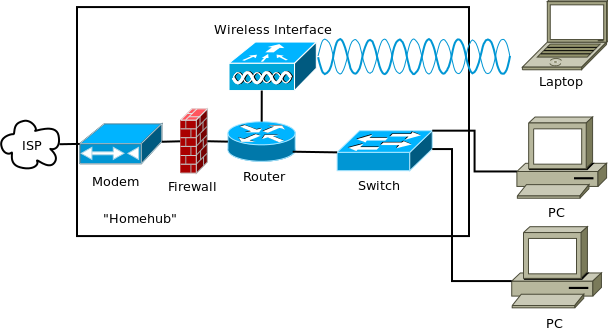
\includegraphics[width=0.75\linewidth]{../Diagrams/Network/TypicalHomenet.png}
\end{center}
This diagram shows a typical home network in the present day. The hardware
inside the box labeled ``Homehub'' is typically provided to customers as one
plug in and play device. It is commonly referred to as a router, although this
is slightly misleading as they perform many other tasks that routing.

As can be seen from the diagram, the box provides the house with wired and
wireless connections to the LAN and the internet. The WLAN is typically bridged
with the LAN to give create a single subnet.

\section{Future}
\label{typical_homenet_future}
\begin{center}
	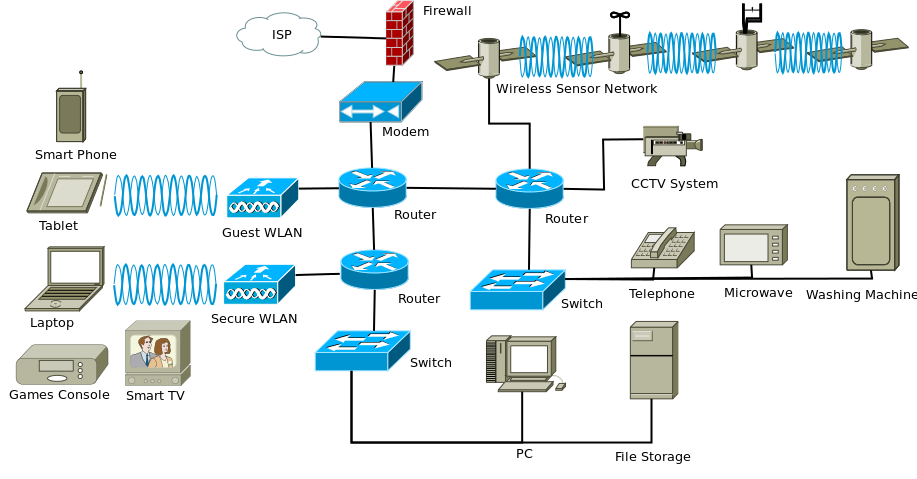
\includegraphics[width=0.9\linewidth]{../Diagrams/Network/FutureHomenet.png}
\end{center}
This diagram shows a hypothetical future home network. The network includes a
guest wireless network, a secured wireless network, a wired network, a network
for appliances, a network for a home surveillance system and a wireless sensor
network.

\chapter{Typical Corporate Network}
\label{typical_coporatenet}
\begin{center}
	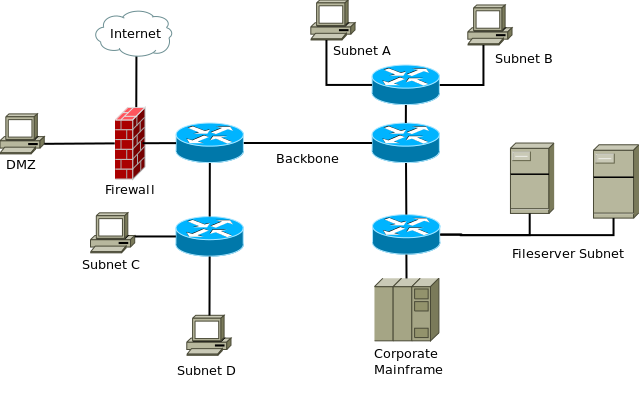
\includegraphics[width=0.5\linewidth]{../Diagrams/Network/CorporateNetwork.png}
\end{center}
This diagram shows the typical topology of a corporate network. For the sake of reducing complexity, Layer 2 switches have not been shown

\end{landscape}


\end{document}
